\documentclass[twoside]{book}

% Packages required by doxygen
\usepackage{fixltx2e}
\usepackage{calc}
\usepackage{doxygen}
\usepackage[export]{adjustbox} % also loads graphicx
\usepackage{graphicx}
\usepackage[utf8]{inputenc}
\usepackage{makeidx}
\usepackage{multicol}
\usepackage{multirow}
\PassOptionsToPackage{warn}{textcomp}
\usepackage{textcomp}
\usepackage[nointegrals]{wasysym}
\usepackage[table]{xcolor}

% Font selection
\usepackage[T1]{fontenc}
\usepackage[scaled=.90]{helvet}
\usepackage{courier}
\usepackage{amssymb}
\usepackage{sectsty}
\renewcommand{\familydefault}{\sfdefault}
\allsectionsfont{%
  \fontseries{bc}\selectfont%
  \color{darkgray}%
}
\renewcommand{\DoxyLabelFont}{%
  \fontseries{bc}\selectfont%
  \color{darkgray}%
}
\newcommand{\+}{\discretionary{\mbox{\scriptsize$\hookleftarrow$}}{}{}}

% Page & text layout
\usepackage{geometry}
\geometry{%
  a4paper,%
  top=2.5cm,%
  bottom=2.5cm,%
  left=2.5cm,%
  right=2.5cm%
}
\tolerance=750
\hfuzz=15pt
\hbadness=750
\setlength{\emergencystretch}{15pt}
\setlength{\parindent}{0cm}
\setlength{\parskip}{0.2cm}
\makeatletter
\renewcommand{\paragraph}{%
  \@startsection{paragraph}{4}{0ex}{-1.0ex}{1.0ex}{%
    \normalfont\normalsize\bfseries\SS@parafont%
  }%
}
\renewcommand{\subparagraph}{%
  \@startsection{subparagraph}{5}{0ex}{-1.0ex}{1.0ex}{%
    \normalfont\normalsize\bfseries\SS@subparafont%
  }%
}
\makeatother

% Headers & footers
\usepackage{fancyhdr}
\pagestyle{fancyplain}
\fancyhead[LE]{\fancyplain{}{\bfseries\thepage}}
\fancyhead[CE]{\fancyplain{}{}}
\fancyhead[RE]{\fancyplain{}{\bfseries\leftmark}}
\fancyhead[LO]{\fancyplain{}{\bfseries\rightmark}}
\fancyhead[CO]{\fancyplain{}{}}
\fancyhead[RO]{\fancyplain{}{\bfseries\thepage}}
\fancyfoot[LE]{\fancyplain{}{}}
\fancyfoot[CE]{\fancyplain{}{}}
\fancyfoot[RE]{\fancyplain{}{\bfseries\scriptsize Generated on Mon Aug 17 2015 17\+:08\+:16 for Dink! by Doxygen }}
\fancyfoot[LO]{\fancyplain{}{\bfseries\scriptsize Generated on Mon Aug 17 2015 17\+:08\+:16 for Dink! by Doxygen }}
\fancyfoot[CO]{\fancyplain{}{}}
\fancyfoot[RO]{\fancyplain{}{}}
\renewcommand{\footrulewidth}{0.4pt}
\renewcommand{\chaptermark}[1]{%
  \markboth{#1}{}%
}
\renewcommand{\sectionmark}[1]{%
  \markright{\thesection\ #1}%
}

% Indices & bibliography
\usepackage{natbib}
\usepackage[titles]{tocloft}
\setcounter{tocdepth}{3}
\setcounter{secnumdepth}{5}
\makeindex

% Hyperlinks (required, but should be loaded last)
\usepackage{ifpdf}
\ifpdf
  \usepackage[pdftex,pagebackref=true]{hyperref}
\else
  \usepackage[ps2pdf,pagebackref=true]{hyperref}
\fi
\hypersetup{%
  colorlinks=true,%
  linkcolor=blue,%
  citecolor=blue,%
  unicode%
}

% Custom commands
\newcommand{\clearemptydoublepage}{%
  \newpage{\pagestyle{empty}\cleardoublepage}%
}


%===== C O N T E N T S =====

\begin{document}

% Titlepage & ToC
\hypersetup{pageanchor=false,
             bookmarks=true,
             bookmarksnumbered=true,
             pdfencoding=unicode
            }
\pagenumbering{roman}
\begin{titlepage}
\vspace*{7cm}
\begin{center}%
{\Large Dink! }\\
\vspace*{1cm}
{\large Generated by Doxygen 1.8.10}\\
\vspace*{0.5cm}
{\small Mon Aug 17 2015 17:08:16}\\
\end{center}
\end{titlepage}
\clearemptydoublepage
\tableofcontents
\clearemptydoublepage
\pagenumbering{arabic}
\hypersetup{pageanchor=true}

%--- Begin generated contents ---
\chapter{Hierarchical Index}
\section{Class Hierarchy}
This inheritance list is sorted roughly, but not completely, alphabetically\+:\begin{DoxyCompactList}
\item \contentsline{section}{Ball}{\pageref{class_ball}}{}
\item \contentsline{section}{Bat}{\pageref{class_bat}}{}
\item \contentsline{section}{Box}{\pageref{class_box}}{}
\item \contentsline{section}{Goal}{\pageref{class_goal}}{}
\item \contentsline{section}{qt\+\_\+meta\+\_\+stringdata\+\_\+\+Open\+G\+L\+Window\+\_\+t}{\pageref{structqt__meta__stringdata___open_g_l_window__t}}{}
\item Q\+Window\begin{DoxyCompactList}
\item \contentsline{section}{Open\+G\+L\+Window}{\pageref{class_open_g_l_window}}{}
\begin{DoxyCompactList}
\item \contentsline{section}{N\+G\+L\+Scene}{\pageref{class_n_g_l_scene}}{}
\end{DoxyCompactList}
\end{DoxyCompactList}
\end{DoxyCompactList}

\chapter{Class Index}
\section{Class List}
Here are the classes, structs, unions and interfaces with brief descriptions\+:\begin{DoxyCompactList}
\item\contentsline{section}{\hyperlink{class_ball}{Ball} \\*The \hyperlink{class_ball}{Ball} class, used to define the ball\textquotesingle{}s attributes and access methods }{\pageref{class_ball}}{}
\item\contentsline{section}{\hyperlink{class_bat}{Bat} \\*The \hyperlink{class_bat}{Bat} class, used to define the bat\textquotesingle{}s attributes and access methods }{\pageref{class_bat}}{}
\item\contentsline{section}{\hyperlink{class_box}{Box} \\*The \hyperlink{class_box}{Box} class, used to define the box\textquotesingle{}s attributes and access methods }{\pageref{class_box}}{}
\item\contentsline{section}{\hyperlink{class_goal}{Goal} \\*The \hyperlink{class_goal}{Goal} class, used to define the goal\textquotesingle{}s attributes and access methods }{\pageref{class_goal}}{}
\item\contentsline{section}{\hyperlink{class_n_g_l_scene}{N\+G\+L\+Scene} \\*Our main glwindow widget for N\+G\+L applications all drawing elements are put in this file }{\pageref{class_n_g_l_scene}}{}
\item\contentsline{section}{\hyperlink{class_open_g_l_window}{Open\+G\+L\+Window} }{\pageref{class_open_g_l_window}}{}
\item\contentsline{section}{\hyperlink{structqt__meta__stringdata___open_g_l_window__t}{qt\+\_\+meta\+\_\+stringdata\+\_\+\+Open\+G\+L\+Window\+\_\+t} }{\pageref{structqt__meta__stringdata___open_g_l_window__t}}{}
\end{DoxyCompactList}

\chapter{File Index}
\section{File List}
Here is a list of all documented files with brief descriptions\+:\begin{DoxyCompactList}
\item\contentsline{section}{include/\hyperlink{_ball_8h}{Ball.\+h} \\*The \hyperlink{class_ball}{Ball} class, used to define the ball\textquotesingle{}s attributes and access methods }{\pageref{_ball_8h}}{}
\item\contentsline{section}{include/\hyperlink{_bat_8h}{Bat.\+h} \\*The \hyperlink{class_bat}{Bat} class, used to define the bat\textquotesingle{}s attributes and access methods }{\pageref{_bat_8h}}{}
\item\contentsline{section}{include/\hyperlink{_box_8h}{Box.\+h} \\*The \hyperlink{class_ball}{Ball} class, used to define the box\textquotesingle{}s attributes and access methods }{\pageref{_box_8h}}{}
\item\contentsline{section}{include/\hyperlink{_goal_8h}{Goal.\+h} \\*The \hyperlink{class_goal}{Goal} class, used to define the goal\textquotesingle{}s attributes and access methods }{\pageref{_goal_8h}}{}
\item\contentsline{section}{include/\hyperlink{_n_g_l_scene_8h}{N\+G\+L\+Scene.\+h} \\*This class inherits from the Qt \hyperlink{class_open_g_l_window}{Open\+G\+L\+Window} and allows us to use N\+G\+L to draw Open\+G\+L }{\pageref{_n_g_l_scene_8h}}{}
\item\contentsline{section}{include/\hyperlink{_open_g_l_window_8h}{Open\+G\+L\+Window.\+h} \\*This is the base class for all our Open\+G\+L widgets, inherit from this class and overide the methods for Open\+G\+L drawing modified from the Qt demo here \href{http://qt-project.org/doc/qt-5.0/qtgui/openglwindow.html}{\tt http\+://qt-\/project.\+org/doc/qt-\/5.\+0/qtgui/openglwindow.\+html} }{\pageref{_open_g_l_window_8h}}{}
\end{DoxyCompactList}

\chapter{Class Documentation}
\hypertarget{class_ball}{}\section{Ball Class Reference}
\label{class_ball}\index{Ball@{Ball}}


The \hyperlink{class_ball}{Ball} class, used to define the ball\textquotesingle{}s attributes and access methods.  




{\ttfamily \#include $<$Ball.\+h$>$}

\subsection*{Public Member Functions}
\begin{DoxyCompactItemize}
\item 
\hypertarget{class_ball_a86a144d3dad6c953e422e32435923bbb}{}\hyperlink{class_ball_a86a144d3dad6c953e422e32435923bbb}{Ball} ()\label{class_ball_a86a144d3dad6c953e422e32435923bbb}

\begin{DoxyCompactList}\small\item\em ctor \end{DoxyCompactList}\item 
void \hyperlink{class_ball_a0b2248494bb869c889847fe7110a6b66}{set\+Position} (const ngl\+::\+Vec3 \+\_\+pos)
\begin{DoxyCompactList}\small\item\em Sets the ball\textquotesingle{}s position. \end{DoxyCompactList}\item 
void \hyperlink{class_ball_abf1da28d789d938eac0f8070e8c35514}{set\+Velocity} (const ngl\+::\+Vec3 \+\_\+v)
\begin{DoxyCompactList}\small\item\em Sets the ball\textquotesingle{}s velocity. \end{DoxyCompactList}\item 
void \hyperlink{class_ball_a01f40cdd20529453aeed3c5a62c480bd}{set\+Radius} (const ngl\+::\+Real \+\_\+r)
\begin{DoxyCompactList}\small\item\em Sets the ball\textquotesingle{}s radius. \end{DoxyCompactList}\item 
\hypertarget{class_ball_adcf84d9f9ae674709c7145b289f2c3b9}{}ngl\+::\+Vec3 \hyperlink{class_ball_adcf84d9f9ae674709c7145b289f2c3b9}{get\+Position} () const \label{class_ball_adcf84d9f9ae674709c7145b289f2c3b9}

\begin{DoxyCompactList}\small\item\em Returns the ball\textquotesingle{}s position. \end{DoxyCompactList}\item 
\hypertarget{class_ball_acea6bc58341f19b42fa3036e07f3e363}{}ngl\+::\+Vec3 \hyperlink{class_ball_acea6bc58341f19b42fa3036e07f3e363}{get\+Velocity} () const \label{class_ball_acea6bc58341f19b42fa3036e07f3e363}

\begin{DoxyCompactList}\small\item\em Returns the ball\textquotesingle{}s velocity. \end{DoxyCompactList}\item 
\hypertarget{class_ball_a27052308f4e776f2c626da88e1b5e840}{}ngl\+::\+Real \hyperlink{class_ball_a27052308f4e776f2c626da88e1b5e840}{get\+Radius} () const \label{class_ball_a27052308f4e776f2c626da88e1b5e840}

\begin{DoxyCompactList}\small\item\em Returns the ball\textquotesingle{}s radius. \end{DoxyCompactList}\item 
\hypertarget{class_ball_a97d273f777a59e0be7ffbf4bef209454}{}ngl\+::\+Material \hyperlink{class_ball_a97d273f777a59e0be7ffbf4bef209454}{get\+Material} () const \label{class_ball_a97d273f777a59e0be7ffbf4bef209454}

\begin{DoxyCompactList}\small\item\em Returns the ball\textquotesingle{}s material. \end{DoxyCompactList}\item 
void \hyperlink{class_ball_a2b9b447d1971e8de179e5e266e37114b}{draw} (const std\+::string \&\+\_\+shader, ngl\+::\+Camera $\ast$\+\_\+cam)
\begin{DoxyCompactList}\small\item\em draws the mesh using the transform stack \end{DoxyCompactList}\item 
void \hyperlink{class_ball_a326e028f9889e8d7900c9d4d0d9f617e}{generate\+Pos} (ngl\+::\+Real \+\_\+box\+Width)
\begin{DoxyCompactList}\small\item\em Uses a random float generator to give the ball a new position. \end{DoxyCompactList}\item 
\hypertarget{class_ball_aca5fc0e9ccbbad1689834d6c364d24b0}{}void \hyperlink{class_ball_aca5fc0e9ccbbad1689834d6c364d24b0}{generate\+Vel} ()\label{class_ball_aca5fc0e9ccbbad1689834d6c364d24b0}

\begin{DoxyCompactList}\small\item\em Uses a random float generator to give the ball a new velocity. \end{DoxyCompactList}\end{DoxyCompactItemize}


\subsection{Detailed Description}
The \hyperlink{class_ball}{Ball} class, used to define the ball\textquotesingle{}s attributes and access methods. 

\subsection{Member Function Documentation}
\hypertarget{class_ball_a2b9b447d1971e8de179e5e266e37114b}{}\index{Ball@{Ball}!draw@{draw}}
\index{draw@{draw}!Ball@{Ball}}
\subsubsection[{draw(const std\+::string \&\+\_\+shader, ngl\+::\+Camera $\ast$\+\_\+cam)}]{\setlength{\rightskip}{0pt plus 5cm}void Ball\+::draw (
\begin{DoxyParamCaption}
\item[{const std\+::string \&}]{\+\_\+shader, }
\item[{ngl\+::\+Camera $\ast$}]{\+\_\+cam}
\end{DoxyParamCaption}
)}\label{class_ball_a2b9b447d1971e8de179e5e266e37114b}


draws the mesh using the transform stack 


\begin{DoxyParams}{Parameters}
{\em \&\+\_\+shader} & the shader used to draw \\
\hline
{\em $\ast$\+\_\+cam} & the viewing camera \\
\hline
\end{DoxyParams}
\hypertarget{class_ball_a326e028f9889e8d7900c9d4d0d9f617e}{}\index{Ball@{Ball}!generate\+Pos@{generate\+Pos}}
\index{generate\+Pos@{generate\+Pos}!Ball@{Ball}}
\subsubsection[{generate\+Pos(ngl\+::\+Real \+\_\+box\+Width)}]{\setlength{\rightskip}{0pt plus 5cm}void Ball\+::generate\+Pos (
\begin{DoxyParamCaption}
\item[{ngl\+::\+Real}]{\+\_\+box\+Width}
\end{DoxyParamCaption}
)}\label{class_ball_a326e028f9889e8d7900c9d4d0d9f617e}


Uses a random float generator to give the ball a new position. 


\begin{DoxyParams}{Parameters}
{\em \+\_\+box\+Width} & width of the box \\
\hline
\end{DoxyParams}
\hypertarget{class_ball_a0b2248494bb869c889847fe7110a6b66}{}\index{Ball@{Ball}!set\+Position@{set\+Position}}
\index{set\+Position@{set\+Position}!Ball@{Ball}}
\subsubsection[{set\+Position(const ngl\+::\+Vec3 \+\_\+pos)}]{\setlength{\rightskip}{0pt plus 5cm}void Ball\+::set\+Position (
\begin{DoxyParamCaption}
\item[{const ngl\+::\+Vec3}]{\+\_\+pos}
\end{DoxyParamCaption}
)\hspace{0.3cm}{\ttfamily [inline]}}\label{class_ball_a0b2248494bb869c889847fe7110a6b66}


Sets the ball\textquotesingle{}s position. 


\begin{DoxyParams}{Parameters}
{\em \+\_\+pos} & the new position \\
\hline
\end{DoxyParams}
\hypertarget{class_ball_a01f40cdd20529453aeed3c5a62c480bd}{}\index{Ball@{Ball}!set\+Radius@{set\+Radius}}
\index{set\+Radius@{set\+Radius}!Ball@{Ball}}
\subsubsection[{set\+Radius(const ngl\+::\+Real \+\_\+r)}]{\setlength{\rightskip}{0pt plus 5cm}void Ball\+::set\+Radius (
\begin{DoxyParamCaption}
\item[{const ngl\+::\+Real}]{\+\_\+r}
\end{DoxyParamCaption}
)\hspace{0.3cm}{\ttfamily [inline]}}\label{class_ball_a01f40cdd20529453aeed3c5a62c480bd}


Sets the ball\textquotesingle{}s radius. 


\begin{DoxyParams}{Parameters}
{\em \+\_\+r} & the new radius \\
\hline
\end{DoxyParams}
\hypertarget{class_ball_abf1da28d789d938eac0f8070e8c35514}{}\index{Ball@{Ball}!set\+Velocity@{set\+Velocity}}
\index{set\+Velocity@{set\+Velocity}!Ball@{Ball}}
\subsubsection[{set\+Velocity(const ngl\+::\+Vec3 \+\_\+v)}]{\setlength{\rightskip}{0pt plus 5cm}void Ball\+::set\+Velocity (
\begin{DoxyParamCaption}
\item[{const ngl\+::\+Vec3}]{\+\_\+v}
\end{DoxyParamCaption}
)\hspace{0.3cm}{\ttfamily [inline]}}\label{class_ball_abf1da28d789d938eac0f8070e8c35514}


Sets the ball\textquotesingle{}s velocity. 


\begin{DoxyParams}{Parameters}
{\em \+\_\+v} & the new velocity \\
\hline
\end{DoxyParams}


The documentation for this class was generated from the following files\+:\begin{DoxyCompactItemize}
\item 
include/\hyperlink{_ball_8h}{Ball.\+h}\item 
src/Ball.\+cpp\end{DoxyCompactItemize}

\hypertarget{class_bat}{}\section{Bat Class Reference}
\label{class_bat}\index{Bat@{Bat}}


The \hyperlink{class_bat}{Bat} class, used to define the bat\textquotesingle{}s attributes and access methods.  




{\ttfamily \#include $<$Bat.\+h$>$}

\subsection*{Public Member Functions}
\begin{DoxyCompactItemize}
\item 
\hypertarget{class_bat_ac231b3a270f82b72dace8be983a6ee6c}{}\hyperlink{class_bat_ac231b3a270f82b72dace8be983a6ee6c}{Bat} ()\label{class_bat_ac231b3a270f82b72dace8be983a6ee6c}

\begin{DoxyCompactList}\small\item\em ctor \end{DoxyCompactList}\item 
void \hyperlink{class_bat_a243a43c23e389b55cb85167fdf657ceb}{set\+Mouse\+Pos} (const ngl\+::\+Vec3 \+\_\+mouse\+Pos)
\begin{DoxyCompactList}\small\item\em Sets the bat\textquotesingle{}s mouse-\/controlled position. \end{DoxyCompactList}\item 
void \hyperlink{class_bat_a17b4c6b2b70a2800a952e16022f47820}{set\+Push\+Pos} (const ngl\+::\+Vec3 \+\_\+push\+Pos)
\begin{DoxyCompactList}\small\item\em Sets the bat\textquotesingle{}s push-\/controlled position. \end{DoxyCompactList}\item 
void \hyperlink{class_bat_a7e7c34ffd00a351cbfbc0c4389bfa43e}{set\+Push\+V} (const ngl\+::\+Vec3 \+\_\+push\+V)
\begin{DoxyCompactList}\small\item\em Sets the bat\textquotesingle{}s push-\/controlled velocity. \end{DoxyCompactList}\item 
void \hyperlink{class_bat_a00e563db4fad9c3a90eb72b5e5e68bc9}{setpush\+A} (const ngl\+::\+Vec3 \+\_\+push\+A)
\begin{DoxyCompactList}\small\item\em Sets the bat\textquotesingle{}s push-\/controlled acceleration. \end{DoxyCompactList}\item 
void \hyperlink{class_bat_a701c00889957e06bd4e78f8e5bc2ec85}{set\+Normal} (const ngl\+::\+Vec3 \+\_\+normal)
\begin{DoxyCompactList}\small\item\em Sets the bat\textquotesingle{}s normal vector. \end{DoxyCompactList}\item 
void \hyperlink{class_bat_acfdb8dcdc698f12a950911f4f7c21995}{set\+Orient} (const ngl\+::\+Vec3 \+\_\+orient)
\begin{DoxyCompactList}\small\item\em Sets the bat\textquotesingle{}s orientation. \end{DoxyCompactList}\item 
void \hyperlink{class_bat_ac7afffdf395f73c1ac05092a81fa863e}{set\+Radius} (const ngl\+::\+Real \+\_\+r)
\begin{DoxyCompactList}\small\item\em Sets the bat\textquotesingle{}s radius. \end{DoxyCompactList}\item 
\hypertarget{class_bat_a7df35992554d7beddebfc3d1a2284891}{}ngl\+::\+Vec3 \hyperlink{class_bat_a7df35992554d7beddebfc3d1a2284891}{get\+Pos} ()\label{class_bat_a7df35992554d7beddebfc3d1a2284891}

\begin{DoxyCompactList}\small\item\em returns the bat\textquotesingle{}s true global position \end{DoxyCompactList}\item 
\hypertarget{class_bat_a84a84c1eaa37f6221282953f93e5b3d8}{}ngl\+::\+Vec3 \hyperlink{class_bat_a84a84c1eaa37f6221282953f93e5b3d8}{get\+Mouse\+Pos} ()\label{class_bat_a84a84c1eaa37f6221282953f93e5b3d8}

\begin{DoxyCompactList}\small\item\em returns the bat\textquotesingle{}s mouse-\/controlled position \end{DoxyCompactList}\item 
\hypertarget{class_bat_a5d2038c9c42d793441795a15c0b0ffce}{}ngl\+::\+Vec3 \hyperlink{class_bat_a5d2038c9c42d793441795a15c0b0ffce}{get\+Mouse\+V} ()\label{class_bat_a5d2038c9c42d793441795a15c0b0ffce}

\begin{DoxyCompactList}\small\item\em returns the bat\textquotesingle{}s mouse-\/controlled velocity \end{DoxyCompactList}\item 
\hypertarget{class_bat_a552c9c5dc6e2fb8e1b3b3ab180d80605}{}ngl\+::\+Vec3 \hyperlink{class_bat_a552c9c5dc6e2fb8e1b3b3ab180d80605}{get\+Normal} ()\label{class_bat_a552c9c5dc6e2fb8e1b3b3ab180d80605}

\begin{DoxyCompactList}\small\item\em returns the bat\textquotesingle{}s normal \end{DoxyCompactList}\item 
\hypertarget{class_bat_a29a52a25985df48a46eca5079e354853}{}ngl\+::\+Vec3 \hyperlink{class_bat_a29a52a25985df48a46eca5079e354853}{get\+Push\+V} ()\label{class_bat_a29a52a25985df48a46eca5079e354853}

\begin{DoxyCompactList}\small\item\em returns the bat\textquotesingle{}s push-\/controlled velocity \end{DoxyCompactList}\item 
\hypertarget{class_bat_afe01a9ede9e614596f408c894e03ca5a}{}ngl\+::\+Vec3 \hyperlink{class_bat_afe01a9ede9e614596f408c894e03ca5a}{get\+Push\+A} ()\label{class_bat_afe01a9ede9e614596f408c894e03ca5a}

\begin{DoxyCompactList}\small\item\em returns the bat\textquotesingle{}s push-\/controlled acceleration \end{DoxyCompactList}\item 
\hypertarget{class_bat_a8ac591209afc830d5f3a904d73efc9bb}{}ngl\+::\+Vec3 \hyperlink{class_bat_a8ac591209afc830d5f3a904d73efc9bb}{get\+Push\+Pos} ()\label{class_bat_a8ac591209afc830d5f3a904d73efc9bb}

\begin{DoxyCompactList}\small\item\em returns the bat\textquotesingle{}s push-\/controlled position \end{DoxyCompactList}\item 
\hypertarget{class_bat_a0a4545f994b1f26ac9ebd1043f0fcb91}{}ngl\+::\+Real \hyperlink{class_bat_a0a4545f994b1f26ac9ebd1043f0fcb91}{get\+Radius} () const \label{class_bat_a0a4545f994b1f26ac9ebd1043f0fcb91}

\begin{DoxyCompactList}\small\item\em returns the bat\textquotesingle{}s radius \end{DoxyCompactList}\item 
\hypertarget{class_bat_a2b91b886a5416294f9a75ea452148b28}{}std\+::string \hyperlink{class_bat_a2b91b886a5416294f9a75ea452148b28}{get\+Push} ()\label{class_bat_a2b91b886a5416294f9a75ea452148b28}

\begin{DoxyCompactList}\small\item\em returns a flag for the state of the push command \end{DoxyCompactList}\item 
\hypertarget{class_bat_a6b799c54fff78b0088831573bb7357bb}{}ngl\+::\+Real \hyperlink{class_bat_a6b799c54fff78b0088831573bb7357bb}{get\+Push\+Dist} ()\label{class_bat_a6b799c54fff78b0088831573bb7357bb}

\begin{DoxyCompactList}\small\item\em returns the limit of the reach of a push \end{DoxyCompactList}\item 
void \hyperlink{class_bat_a07907b3c6e056575b2b20fcbf2d6c679}{draw} (const std\+::string \&\+\_\+shader, ngl\+::\+Camera $\ast$\+\_\+cam)
\begin{DoxyCompactList}\small\item\em draws the bat \end{DoxyCompactList}\item 
\hypertarget{class_bat_a6012876b0637a7867b3256296dd74f48}{}void \hyperlink{class_bat_a6012876b0637a7867b3256296dd74f48}{push\+Start} ()\label{class_bat_a6012876b0637a7867b3256296dd74f48}

\begin{DoxyCompactList}\small\item\em initiates the push command \end{DoxyCompactList}\item 
\hypertarget{class_bat_a2e9d58e022c3a3871c66a35b6e150740}{}void \hyperlink{class_bat_a2e9d58e022c3a3871c66a35b6e150740}{push\+Peak} ()\label{class_bat_a2e9d58e022c3a3871c66a35b6e150740}

\begin{DoxyCompactList}\small\item\em initiated when bat has reached push limit \end{DoxyCompactList}\item 
\hypertarget{class_bat_a9e29871261f3bfec5c8cc5f5e2805815}{}void \hyperlink{class_bat_a9e29871261f3bfec5c8cc5f5e2805815}{push\+Stop} ()\label{class_bat_a9e29871261f3bfec5c8cc5f5e2805815}

\begin{DoxyCompactList}\small\item\em completes the push and returns mouse control \end{DoxyCompactList}\end{DoxyCompactItemize}


\subsection{Detailed Description}
The \hyperlink{class_bat}{Bat} class, used to define the bat\textquotesingle{}s attributes and access methods. 

\subsection{Member Function Documentation}
\hypertarget{class_bat_a07907b3c6e056575b2b20fcbf2d6c679}{}\index{Bat@{Bat}!draw@{draw}}
\index{draw@{draw}!Bat@{Bat}}
\subsubsection[{draw(const std\+::string \&\+\_\+shader, ngl\+::\+Camera $\ast$\+\_\+cam)}]{\setlength{\rightskip}{0pt plus 5cm}void Bat\+::draw (
\begin{DoxyParamCaption}
\item[{const std\+::string \&}]{\+\_\+shader, }
\item[{ngl\+::\+Camera $\ast$}]{\+\_\+cam}
\end{DoxyParamCaption}
)}\label{class_bat_a07907b3c6e056575b2b20fcbf2d6c679}


draws the bat 


\begin{DoxyParams}{Parameters}
{\em \&\+\_\+shader} & the shader used to draw \\
\hline
{\em $\ast$\+\_\+cam} & the viewing camera \\
\hline
\end{DoxyParams}
\hypertarget{class_bat_a243a43c23e389b55cb85167fdf657ceb}{}\index{Bat@{Bat}!set\+Mouse\+Pos@{set\+Mouse\+Pos}}
\index{set\+Mouse\+Pos@{set\+Mouse\+Pos}!Bat@{Bat}}
\subsubsection[{set\+Mouse\+Pos(const ngl\+::\+Vec3 \+\_\+mouse\+Pos)}]{\setlength{\rightskip}{0pt plus 5cm}void Bat\+::set\+Mouse\+Pos (
\begin{DoxyParamCaption}
\item[{const ngl\+::\+Vec3}]{\+\_\+mouse\+Pos}
\end{DoxyParamCaption}
)\hspace{0.3cm}{\ttfamily [inline]}}\label{class_bat_a243a43c23e389b55cb85167fdf657ceb}


Sets the bat\textquotesingle{}s mouse-\/controlled position. 


\begin{DoxyParams}{Parameters}
{\em \+\_\+mouse\+Pos} & the new position \\
\hline
\end{DoxyParams}
\hypertarget{class_bat_a701c00889957e06bd4e78f8e5bc2ec85}{}\index{Bat@{Bat}!set\+Normal@{set\+Normal}}
\index{set\+Normal@{set\+Normal}!Bat@{Bat}}
\subsubsection[{set\+Normal(const ngl\+::\+Vec3 \+\_\+normal)}]{\setlength{\rightskip}{0pt plus 5cm}void Bat\+::set\+Normal (
\begin{DoxyParamCaption}
\item[{const ngl\+::\+Vec3}]{\+\_\+normal}
\end{DoxyParamCaption}
)\hspace{0.3cm}{\ttfamily [inline]}}\label{class_bat_a701c00889957e06bd4e78f8e5bc2ec85}


Sets the bat\textquotesingle{}s normal vector. 


\begin{DoxyParams}{Parameters}
{\em \+\_\+normal} & the new normal vector \\
\hline
\end{DoxyParams}
\hypertarget{class_bat_acfdb8dcdc698f12a950911f4f7c21995}{}\index{Bat@{Bat}!set\+Orient@{set\+Orient}}
\index{set\+Orient@{set\+Orient}!Bat@{Bat}}
\subsubsection[{set\+Orient(const ngl\+::\+Vec3 \+\_\+orient)}]{\setlength{\rightskip}{0pt plus 5cm}void Bat\+::set\+Orient (
\begin{DoxyParamCaption}
\item[{const ngl\+::\+Vec3}]{\+\_\+orient}
\end{DoxyParamCaption}
)\hspace{0.3cm}{\ttfamily [inline]}}\label{class_bat_acfdb8dcdc698f12a950911f4f7c21995}


Sets the bat\textquotesingle{}s orientation. 


\begin{DoxyParams}{Parameters}
{\em \+\_\+orient} & the new orientation \\
\hline
\end{DoxyParams}
\hypertarget{class_bat_a00e563db4fad9c3a90eb72b5e5e68bc9}{}\index{Bat@{Bat}!setpush\+A@{setpush\+A}}
\index{setpush\+A@{setpush\+A}!Bat@{Bat}}
\subsubsection[{setpush\+A(const ngl\+::\+Vec3 \+\_\+push\+A)}]{\setlength{\rightskip}{0pt plus 5cm}void Bat\+::setpush\+A (
\begin{DoxyParamCaption}
\item[{const ngl\+::\+Vec3}]{\+\_\+push\+A}
\end{DoxyParamCaption}
)\hspace{0.3cm}{\ttfamily [inline]}}\label{class_bat_a00e563db4fad9c3a90eb72b5e5e68bc9}


Sets the bat\textquotesingle{}s push-\/controlled acceleration. 


\begin{DoxyParams}{Parameters}
{\em \+\_\+push\+A} & the new acceleration \\
\hline
\end{DoxyParams}
\hypertarget{class_bat_a17b4c6b2b70a2800a952e16022f47820}{}\index{Bat@{Bat}!set\+Push\+Pos@{set\+Push\+Pos}}
\index{set\+Push\+Pos@{set\+Push\+Pos}!Bat@{Bat}}
\subsubsection[{set\+Push\+Pos(const ngl\+::\+Vec3 \+\_\+push\+Pos)}]{\setlength{\rightskip}{0pt plus 5cm}void Bat\+::set\+Push\+Pos (
\begin{DoxyParamCaption}
\item[{const ngl\+::\+Vec3}]{\+\_\+push\+Pos}
\end{DoxyParamCaption}
)\hspace{0.3cm}{\ttfamily [inline]}}\label{class_bat_a17b4c6b2b70a2800a952e16022f47820}


Sets the bat\textquotesingle{}s push-\/controlled position. 


\begin{DoxyParams}{Parameters}
{\em \+\_\+push\+Pos} & the new position \\
\hline
\end{DoxyParams}
\hypertarget{class_bat_a7e7c34ffd00a351cbfbc0c4389bfa43e}{}\index{Bat@{Bat}!set\+Push\+V@{set\+Push\+V}}
\index{set\+Push\+V@{set\+Push\+V}!Bat@{Bat}}
\subsubsection[{set\+Push\+V(const ngl\+::\+Vec3 \+\_\+push\+V)}]{\setlength{\rightskip}{0pt plus 5cm}void Bat\+::set\+Push\+V (
\begin{DoxyParamCaption}
\item[{const ngl\+::\+Vec3}]{\+\_\+push\+V}
\end{DoxyParamCaption}
)\hspace{0.3cm}{\ttfamily [inline]}}\label{class_bat_a7e7c34ffd00a351cbfbc0c4389bfa43e}


Sets the bat\textquotesingle{}s push-\/controlled velocity. 


\begin{DoxyParams}{Parameters}
{\em \+\_\+push\+V} & the new velocity \\
\hline
\end{DoxyParams}
\hypertarget{class_bat_ac7afffdf395f73c1ac05092a81fa863e}{}\index{Bat@{Bat}!set\+Radius@{set\+Radius}}
\index{set\+Radius@{set\+Radius}!Bat@{Bat}}
\subsubsection[{set\+Radius(const ngl\+::\+Real \+\_\+r)}]{\setlength{\rightskip}{0pt plus 5cm}void Bat\+::set\+Radius (
\begin{DoxyParamCaption}
\item[{const ngl\+::\+Real}]{\+\_\+r}
\end{DoxyParamCaption}
)\hspace{0.3cm}{\ttfamily [inline]}}\label{class_bat_ac7afffdf395f73c1ac05092a81fa863e}


Sets the bat\textquotesingle{}s radius. 


\begin{DoxyParams}{Parameters}
{\em \+\_\+r} & the new radius \\
\hline
\end{DoxyParams}


The documentation for this class was generated from the following files\+:\begin{DoxyCompactItemize}
\item 
include/\hyperlink{_bat_8h}{Bat.\+h}\item 
src/Bat.\+cpp\end{DoxyCompactItemize}

\hypertarget{class_box}{}\section{Box Class Reference}
\label{class_box}\index{Box@{Box}}


The \hyperlink{class_box}{Box} class, used to define the box\textquotesingle{}s attributes and access methods.  




{\ttfamily \#include $<$Box.\+h$>$}

\subsection*{Public Member Functions}
\begin{DoxyCompactItemize}
\item 
\hypertarget{class_box_aca78d7db44972bfa78d46b7bbc8796f6}{}\hyperlink{class_box_aca78d7db44972bfa78d46b7bbc8796f6}{Box} ()\label{class_box_aca78d7db44972bfa78d46b7bbc8796f6}

\begin{DoxyCompactList}\small\item\em ctor \end{DoxyCompactList}\item 
\hypertarget{class_box_a00b3e37cb5fba4097557ea9d9074d89f}{}ngl\+::\+Real \hyperlink{class_box_a00b3e37cb5fba4097557ea9d9074d89f}{get\+Width} ()\label{class_box_a00b3e37cb5fba4097557ea9d9074d89f}

\begin{DoxyCompactList}\small\item\em returns the box\textquotesingle{}s width \end{DoxyCompactList}\item 
\hypertarget{class_box_abc7c98fba087aceb295cf1629eab6450}{}ngl\+::\+Real \hyperlink{class_box_abc7c98fba087aceb295cf1629eab6450}{get\+Height} ()\label{class_box_abc7c98fba087aceb295cf1629eab6450}

\begin{DoxyCompactList}\small\item\em returns the box\textquotesingle{}s height \end{DoxyCompactList}\item 
\hypertarget{class_box_af8499ad434a289212dd226ed540e1180}{}ngl\+::\+Real \hyperlink{class_box_af8499ad434a289212dd226ed540e1180}{get\+Depth} ()\label{class_box_af8499ad434a289212dd226ed540e1180}

\begin{DoxyCompactList}\small\item\em returns the box\textquotesingle{}s depth \end{DoxyCompactList}\item 
void \hyperlink{class_box_adb7764c39ba17be6c83364c8284c263a}{draw} (const std\+::string \&\+\_\+shader, ngl\+::\+Camera $\ast$\+\_\+cam)
\begin{DoxyCompactList}\small\item\em draws the box\textquotesingle{}s mesh using the transform stack \end{DoxyCompactList}\end{DoxyCompactItemize}


\subsection{Detailed Description}
The \hyperlink{class_box}{Box} class, used to define the box\textquotesingle{}s attributes and access methods. 

\subsection{Member Function Documentation}
\hypertarget{class_box_adb7764c39ba17be6c83364c8284c263a}{}\index{Box@{Box}!draw@{draw}}
\index{draw@{draw}!Box@{Box}}
\subsubsection[{draw(const std\+::string \&\+\_\+shader, ngl\+::\+Camera $\ast$\+\_\+cam)}]{\setlength{\rightskip}{0pt plus 5cm}void Box\+::draw (
\begin{DoxyParamCaption}
\item[{const std\+::string \&}]{\+\_\+shader, }
\item[{ngl\+::\+Camera $\ast$}]{\+\_\+cam}
\end{DoxyParamCaption}
)}\label{class_box_adb7764c39ba17be6c83364c8284c263a}


draws the box\textquotesingle{}s mesh using the transform stack 


\begin{DoxyParams}{Parameters}
{\em \&\+\_\+shader} & the shader used to draw \\
\hline
{\em $\ast$\+\_\+cam} & the viewing camera \\
\hline
\end{DoxyParams}


The documentation for this class was generated from the following files\+:\begin{DoxyCompactItemize}
\item 
include/\hyperlink{_box_8h}{Box.\+h}\item 
src/Box.\+cpp\end{DoxyCompactItemize}

\hypertarget{class_goal}{}\section{Goal Class Reference}
\label{class_goal}\index{Goal@{Goal}}


The \hyperlink{class_goal}{Goal} class, used to define the goal\textquotesingle{}s attributes and access methods.  




{\ttfamily \#include $<$Goal.\+h$>$}

\subsection*{Public Member Functions}
\begin{DoxyCompactItemize}
\item 
\hypertarget{class_goal_aef5013c9bf548e51178f58da869d508a}{}\hyperlink{class_goal_aef5013c9bf548e51178f58da869d508a}{Goal} ()\label{class_goal_aef5013c9bf548e51178f58da869d508a}

\begin{DoxyCompactList}\small\item\em ctor \end{DoxyCompactList}\item 
\hypertarget{class_goal_a41b52fb4aed63337a5894f986b8c40ee}{}ngl\+::\+Real \hyperlink{class_goal_a41b52fb4aed63337a5894f986b8c40ee}{get\+Radius} ()\label{class_goal_a41b52fb4aed63337a5894f986b8c40ee}

\begin{DoxyCompactList}\small\item\em returns the scale of the goal \end{DoxyCompactList}\item 
\hypertarget{class_goal_a638ba69f64454e4020b6de63f5ed48eb}{}ngl\+::\+Vec3 \hyperlink{class_goal_a638ba69f64454e4020b6de63f5ed48eb}{get\+Position} ()\label{class_goal_a638ba69f64454e4020b6de63f5ed48eb}

\begin{DoxyCompactList}\small\item\em returns the position of the goal \end{DoxyCompactList}\item 
void \hyperlink{class_goal_ae1086a08dc341ee6c75141fc2fa7a7ce}{draw} (const std\+::string \&\+\_\+shader, ngl\+::\+Camera $\ast$\+\_\+cam)
\begin{DoxyCompactList}\small\item\em draws the mesh using the transform stack \end{DoxyCompactList}\item 
void \hyperlink{class_goal_a8258795f65e20e894229ecccd5109411}{generate\+Pos} (ngl\+::\+Real \+\_\+box\+Width, ngl\+::\+Real \+\_\+box\+Height, ngl\+::\+Real \+\_\+box\+Depth)
\begin{DoxyCompactList}\small\item\em Uses a random float generator to give the goal a new position. \end{DoxyCompactList}\item 
void \hyperlink{class_goal_aac120704787f96925565b70ff073af38}{increase\+Difficulty} (const int \+\_\+current\+Score)
\begin{DoxyCompactList}\small\item\em changes the scale of the goal \end{DoxyCompactList}\end{DoxyCompactItemize}


\subsection{Detailed Description}
The \hyperlink{class_goal}{Goal} class, used to define the goal\textquotesingle{}s attributes and access methods. 

\subsection{Member Function Documentation}
\hypertarget{class_goal_ae1086a08dc341ee6c75141fc2fa7a7ce}{}\index{Goal@{Goal}!draw@{draw}}
\index{draw@{draw}!Goal@{Goal}}
\subsubsection[{draw(const std\+::string \&\+\_\+shader, ngl\+::\+Camera $\ast$\+\_\+cam)}]{\setlength{\rightskip}{0pt plus 5cm}void Goal\+::draw (
\begin{DoxyParamCaption}
\item[{const std\+::string \&}]{\+\_\+shader, }
\item[{ngl\+::\+Camera $\ast$}]{\+\_\+cam}
\end{DoxyParamCaption}
)}\label{class_goal_ae1086a08dc341ee6c75141fc2fa7a7ce}


draws the mesh using the transform stack 


\begin{DoxyParams}{Parameters}
{\em \&\+\_\+shader} & the shader used to draw \\
\hline
{\em $\ast$\+\_\+cam} & the viewing camera \\
\hline
\end{DoxyParams}
\hypertarget{class_goal_a8258795f65e20e894229ecccd5109411}{}\index{Goal@{Goal}!generate\+Pos@{generate\+Pos}}
\index{generate\+Pos@{generate\+Pos}!Goal@{Goal}}
\subsubsection[{generate\+Pos(ngl\+::\+Real \+\_\+box\+Width, ngl\+::\+Real \+\_\+box\+Height, ngl\+::\+Real \+\_\+box\+Depth)}]{\setlength{\rightskip}{0pt plus 5cm}void Goal\+::generate\+Pos (
\begin{DoxyParamCaption}
\item[{ngl\+::\+Real}]{\+\_\+box\+Width, }
\item[{ngl\+::\+Real}]{\+\_\+box\+Height, }
\item[{ngl\+::\+Real}]{\+\_\+box\+Depth}
\end{DoxyParamCaption}
)}\label{class_goal_a8258795f65e20e894229ecccd5109411}


Uses a random float generator to give the goal a new position. 


\begin{DoxyParams}{Parameters}
{\em \+\_\+box\+Width} & width of the box \\
\hline
{\em \+\_\+box\+Height} & height of the box \\
\hline
{\em \+\_\+box\+Depth} & depth of the box \\
\hline
\end{DoxyParams}
\hypertarget{class_goal_aac120704787f96925565b70ff073af38}{}\index{Goal@{Goal}!increase\+Difficulty@{increase\+Difficulty}}
\index{increase\+Difficulty@{increase\+Difficulty}!Goal@{Goal}}
\subsubsection[{increase\+Difficulty(const int \+\_\+current\+Score)}]{\setlength{\rightskip}{0pt plus 5cm}void Goal\+::increase\+Difficulty (
\begin{DoxyParamCaption}
\item[{const int}]{\+\_\+current\+Score}
\end{DoxyParamCaption}
)}\label{class_goal_aac120704787f96925565b70ff073af38}


changes the scale of the goal 


\begin{DoxyParams}{Parameters}
{\em the} & current score \\
\hline
\end{DoxyParams}


The documentation for this class was generated from the following files\+:\begin{DoxyCompactItemize}
\item 
include/\hyperlink{_goal_8h}{Goal.\+h}\item 
src/Goal.\+cpp\end{DoxyCompactItemize}

\hypertarget{class_n_g_l_scene}{}\section{N\+G\+L\+Scene Class Reference}
\label{class_n_g_l_scene}\index{N\+G\+L\+Scene@{N\+G\+L\+Scene}}


our main glwindow widget for N\+G\+L applications all drawing elements are put in this file  




{\ttfamily \#include $<$N\+G\+L\+Scene.\+h$>$}

Inheritance diagram for N\+G\+L\+Scene\+:\begin{figure}[H]
\begin{center}
\leavevmode
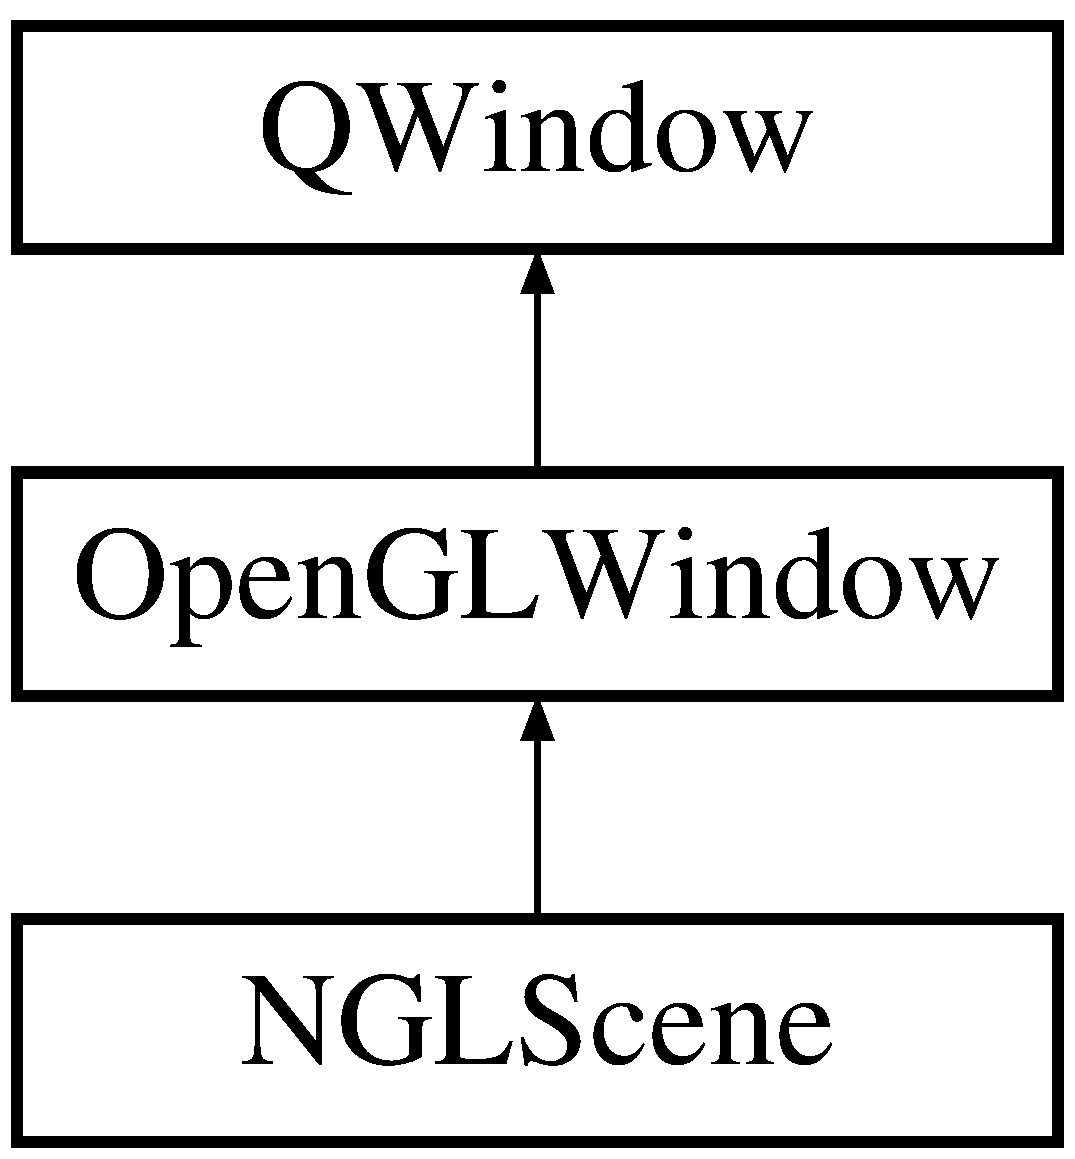
\includegraphics[height=3.000000cm]{class_n_g_l_scene}
\end{center}
\end{figure}
\subsection*{Public Member Functions}
\begin{DoxyCompactItemize}
\item 
\hyperlink{class_n_g_l_scene_adbde5986bed766df177e33baa7fbb222}{N\+G\+L\+Scene} (Q\+Window $\ast$\+\_\+parent=0)
\begin{DoxyCompactList}\small\item\em ctor for our N\+G\+L drawing class \end{DoxyCompactList}\item 
\hypertarget{class_n_g_l_scene_abda05d130945833bfbb6bad8d619f7f5}{}\hyperlink{class_n_g_l_scene_abda05d130945833bfbb6bad8d619f7f5}{$\sim$\+N\+G\+L\+Scene} ()\label{class_n_g_l_scene_abda05d130945833bfbb6bad8d619f7f5}

\begin{DoxyCompactList}\small\item\em dtor must close down ngl and release Open\+G\+L resources \end{DoxyCompactList}\item 
\hypertarget{class_n_g_l_scene_a63e57fc201b639e51c6eed6ec3b6b992}{}void \hyperlink{class_n_g_l_scene_a63e57fc201b639e51c6eed6ec3b6b992}{initialize} ()\label{class_n_g_l_scene_a63e57fc201b639e51c6eed6ec3b6b992}

\begin{DoxyCompactList}\small\item\em the initialize class is called once when the window is created and we have a valid G\+L context use this to setup any default G\+L stuff \end{DoxyCompactList}\item 
\hypertarget{class_n_g_l_scene_a63905ed5bab957d8e2d5528f942feb42}{}void \hyperlink{class_n_g_l_scene_a63905ed5bab957d8e2d5528f942feb42}{render} ()\label{class_n_g_l_scene_a63905ed5bab957d8e2d5528f942feb42}

\begin{DoxyCompactList}\small\item\em this is called everytime we want to draw the scene \end{DoxyCompactList}\end{DoxyCompactItemize}
\subsection*{Additional Inherited Members}


\subsection{Detailed Description}
our main glwindow widget for N\+G\+L applications all drawing elements are put in this file 

\subsection{Constructor \& Destructor Documentation}
\hypertarget{class_n_g_l_scene_adbde5986bed766df177e33baa7fbb222}{}\index{N\+G\+L\+Scene@{N\+G\+L\+Scene}!N\+G\+L\+Scene@{N\+G\+L\+Scene}}
\index{N\+G\+L\+Scene@{N\+G\+L\+Scene}!N\+G\+L\+Scene@{N\+G\+L\+Scene}}
\subsubsection[{N\+G\+L\+Scene(\+Q\+Window $\ast$\+\_\+parent=0)}]{\setlength{\rightskip}{0pt plus 5cm}N\+G\+L\+Scene\+::\+N\+G\+L\+Scene (
\begin{DoxyParamCaption}
\item[{Q\+Window $\ast$}]{\+\_\+parent = {\ttfamily 0}}
\end{DoxyParamCaption}
)}\label{class_n_g_l_scene_adbde5986bed766df177e33baa7fbb222}


ctor for our N\+G\+L drawing class 


\begin{DoxyParams}[1]{Parameters}
\mbox{\tt in}  & {\em parent} & the parent window to the class \\
\hline
\end{DoxyParams}


The documentation for this class was generated from the following files\+:\begin{DoxyCompactItemize}
\item 
include/\hyperlink{_n_g_l_scene_8h}{N\+G\+L\+Scene.\+h}\item 
src/N\+G\+L\+Scene.\+cpp\end{DoxyCompactItemize}

\hypertarget{class_open_g_l_window}{}\section{Open\+G\+L\+Window Class Reference}
\label{class_open_g_l_window}\index{Open\+G\+L\+Window@{Open\+G\+L\+Window}}
Inheritance diagram for Open\+G\+L\+Window\+:\begin{figure}[H]
\begin{center}
\leavevmode
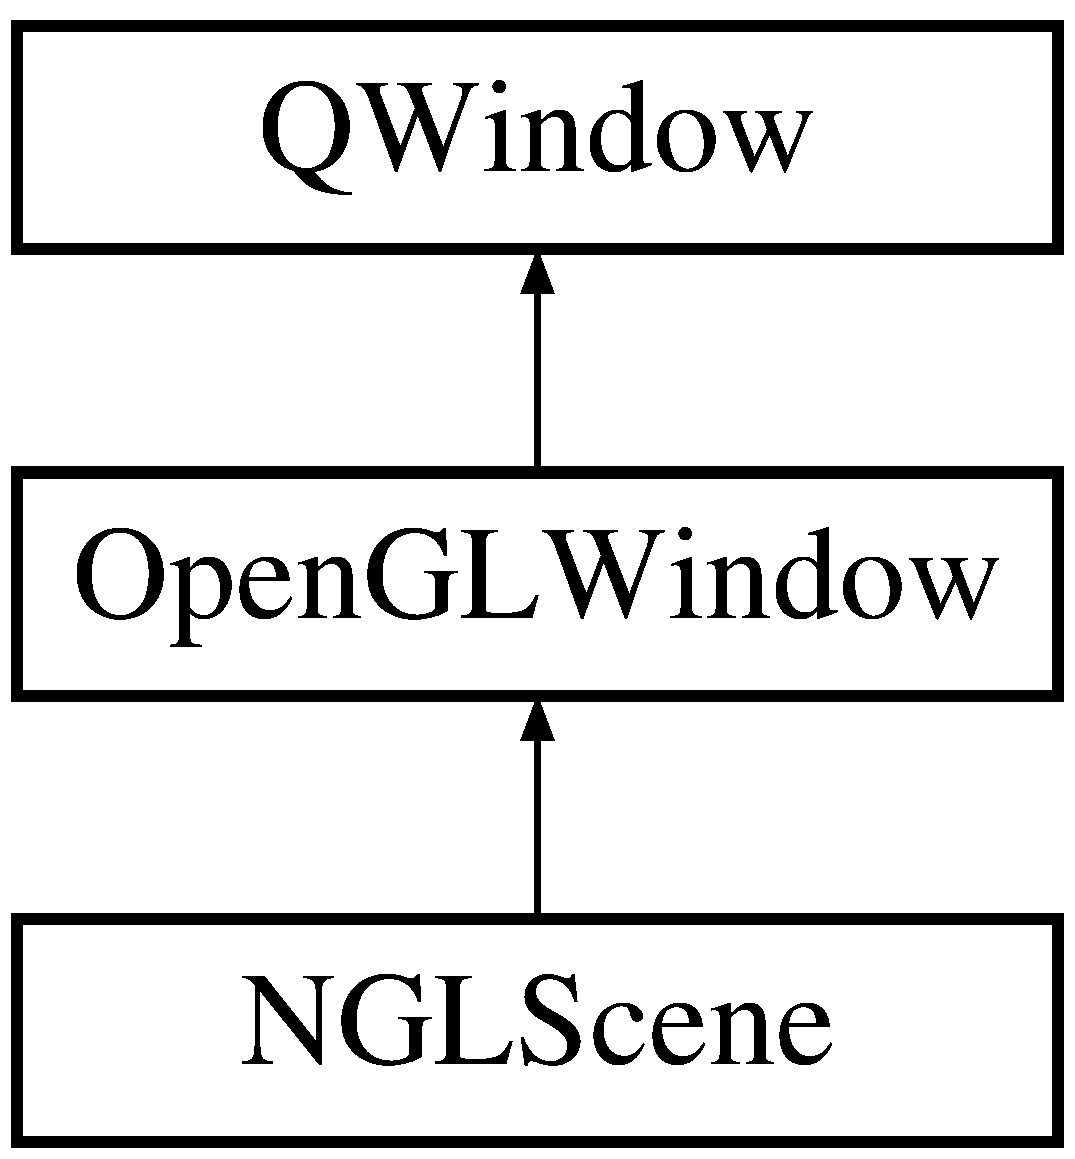
\includegraphics[height=3.000000cm]{class_open_g_l_window}
\end{center}
\end{figure}
\subsection*{Public Slots}
\begin{DoxyCompactItemize}
\item 
\hypertarget{class_open_g_l_window_abea9e50147496e5110b86f03122fbece}{}void \hyperlink{class_open_g_l_window_abea9e50147496e5110b86f03122fbece}{render\+Later} ()\label{class_open_g_l_window_abea9e50147496e5110b86f03122fbece}

\begin{DoxyCompactList}\small\item\em Qt slot to allow use to queue up a render for the next avaliable event process. \end{DoxyCompactList}\item 
\hypertarget{class_open_g_l_window_a8398ed62d646739fe54fae94c477ad1d}{}void \hyperlink{class_open_g_l_window_a8398ed62d646739fe54fae94c477ad1d}{render\+Now} ()\label{class_open_g_l_window_a8398ed62d646739fe54fae94c477ad1d}

\begin{DoxyCompactList}\small\item\em slot to tell us to render immediatly \end{DoxyCompactList}\end{DoxyCompactItemize}
\subsection*{Public Member Functions}
\begin{DoxyCompactItemize}
\item 
\hyperlink{class_open_g_l_window_a2fd92afd17361a60e058dc5433c316af}{Open\+G\+L\+Window} (Q\+Window $\ast$\+\_\+parent=0)
\begin{DoxyCompactList}\small\item\em ctor for Open\+G\+L window must set the surface type to Open\+G\+L \end{DoxyCompactList}\item 
\hypertarget{class_open_g_l_window_aa220b192c71871aab9100f4058a8d62d}{}\hyperlink{class_open_g_l_window_aa220b192c71871aab9100f4058a8d62d}{$\sim$\+Open\+G\+L\+Window} ()\label{class_open_g_l_window_aa220b192c71871aab9100f4058a8d62d}

\begin{DoxyCompactList}\small\item\em dtor, remember to remove the device once finished \end{DoxyCompactList}\item 
\hypertarget{class_open_g_l_window_a0e0194a4f0a30af7249819094c7d1d35}{}virtual void \hyperlink{class_open_g_l_window_a0e0194a4f0a30af7249819094c7d1d35}{render} ()=0\label{class_open_g_l_window_a0e0194a4f0a30af7249819094c7d1d35}

\begin{DoxyCompactList}\small\item\em pure virtual render method we override in our base class to do our drawing, called every update \end{DoxyCompactList}\item 
\hypertarget{class_open_g_l_window_a00b6a24198503b88aea4c5a995723db2}{}virtual void \hyperlink{class_open_g_l_window_a00b6a24198503b88aea4c5a995723db2}{initialize} ()=0\label{class_open_g_l_window_a00b6a24198503b88aea4c5a995723db2}

\begin{DoxyCompactList}\small\item\em pure virtual initialize method we override in our base class to do our drawing this is only called one time, just after we have a valid G\+L context use this to init any global G\+L elements \end{DoxyCompactList}\end{DoxyCompactItemize}
\subsection*{Protected Member Functions}
\begin{DoxyCompactItemize}
\item 
\hypertarget{class_open_g_l_window_a1e3045cffb900de55b7384f5091c9d94}{}bool \hyperlink{class_open_g_l_window_a1e3045cffb900de55b7384f5091c9d94}{event} (Q\+Event $\ast$event)\label{class_open_g_l_window_a1e3045cffb900de55b7384f5091c9d94}

\begin{DoxyCompactList}\small\item\em qt event processing if we post render\+Later event this will be called and execute a render \end{DoxyCompactList}\item 
\hypertarget{class_open_g_l_window_a991121ba7a4bbfa208fa74e5c86004c3}{}void \hyperlink{class_open_g_l_window_a991121ba7a4bbfa208fa74e5c86004c3}{expose\+Event} (Q\+Expose\+Event $\ast$\hyperlink{class_open_g_l_window_a1e3045cffb900de55b7384f5091c9d94}{event})\label{class_open_g_l_window_a991121ba7a4bbfa208fa74e5c86004c3}

\begin{DoxyCompactList}\small\item\em this even is called when the window is made visible and will trigger a render \end{DoxyCompactList}\end{DoxyCompactItemize}


\subsection{Constructor \& Destructor Documentation}
\hypertarget{class_open_g_l_window_a2fd92afd17361a60e058dc5433c316af}{}\index{Open\+G\+L\+Window@{Open\+G\+L\+Window}!Open\+G\+L\+Window@{Open\+G\+L\+Window}}
\index{Open\+G\+L\+Window@{Open\+G\+L\+Window}!Open\+G\+L\+Window@{Open\+G\+L\+Window}}
\subsubsection[{Open\+G\+L\+Window(\+Q\+Window $\ast$\+\_\+parent=0)}]{\setlength{\rightskip}{0pt plus 5cm}Open\+G\+L\+Window\+::\+Open\+G\+L\+Window (
\begin{DoxyParamCaption}
\item[{Q\+Window $\ast$}]{\+\_\+parent = {\ttfamily 0}}
\end{DoxyParamCaption}
)\hspace{0.3cm}{\ttfamily [explicit]}}\label{class_open_g_l_window_a2fd92afd17361a60e058dc5433c316af}


ctor for Open\+G\+L window must set the surface type to Open\+G\+L 


\begin{DoxyParams}[1]{Parameters}
\mbox{\tt in}  & {\em parent} & the parent window to the class \\
\hline
\end{DoxyParams}


The documentation for this class was generated from the following files\+:\begin{DoxyCompactItemize}
\item 
include/\hyperlink{_open_g_l_window_8h}{Open\+G\+L\+Window.\+h}\item 
src/Open\+G\+L\+Window.\+cpp\end{DoxyCompactItemize}

\hypertarget{structqt__meta__stringdata___open_g_l_window__t}{}\section{qt\+\_\+meta\+\_\+stringdata\+\_\+\+Open\+G\+L\+Window\+\_\+t Struct Reference}
\label{structqt__meta__stringdata___open_g_l_window__t}\index{qt\+\_\+meta\+\_\+stringdata\+\_\+\+Open\+G\+L\+Window\+\_\+t@{qt\+\_\+meta\+\_\+stringdata\+\_\+\+Open\+G\+L\+Window\+\_\+t}}
\subsection*{Public Attributes}
\begin{DoxyCompactItemize}
\item 
\hypertarget{structqt__meta__stringdata___open_g_l_window__t_a446763ab1eb9735ae0e4d708155ba912}{}Q\+Byte\+Array\+Data {\bfseries data} \mbox{[}4\mbox{]}\label{structqt__meta__stringdata___open_g_l_window__t_a446763ab1eb9735ae0e4d708155ba912}

\item 
\hypertarget{structqt__meta__stringdata___open_g_l_window__t_ac370b4e76c7d7c54bef1d5592a64fa47}{}char {\bfseries stringdata} \mbox{[}36\mbox{]}\label{structqt__meta__stringdata___open_g_l_window__t_ac370b4e76c7d7c54bef1d5592a64fa47}

\end{DoxyCompactItemize}


The documentation for this struct was generated from the following file\+:\begin{DoxyCompactItemize}
\item 
moc/moc\+\_\+\+Open\+G\+L\+Window.\+cpp\end{DoxyCompactItemize}

\chapter{File Documentation}
\hypertarget{_ball_8h}{}\section{include/\+Ball.h File Reference}
\label{_ball_8h}\index{include/\+Ball.\+h@{include/\+Ball.\+h}}


The \hyperlink{class_ball}{Ball} class, used to define the ball\textquotesingle{}s attributes and access methods.  


{\ttfamily \#include $<$ngl/\+Camera.\+h$>$}\\*
{\ttfamily \#include $<$ngl/\+Vec3.\+h$>$}\\*
{\ttfamily \#include $<$ngl/\+Obj.\+h$>$}\\*
{\ttfamily \#include $<$ngl/\+Transformation.\+h$>$}\\*
{\ttfamily \#include $<$ngl/\+Material.\+h$>$}\\*
{\ttfamily \#include $<$stdlib.\+h$>$}\\*
{\ttfamily \#include $<$random$>$}\\*
{\ttfamily \#include $<$time.\+h$>$}\\*
\subsection*{Classes}
\begin{DoxyCompactItemize}
\item 
class \hyperlink{class_ball}{Ball}
\begin{DoxyCompactList}\small\item\em The \hyperlink{class_ball}{Ball} class, used to define the ball\textquotesingle{}s attributes and access methods. \end{DoxyCompactList}\end{DoxyCompactItemize}


\subsection{Detailed Description}
The \hyperlink{class_ball}{Ball} class, used to define the ball\textquotesingle{}s attributes and access methods. 

\begin{DoxyAuthor}{Author}
Vincent Clifton 
\end{DoxyAuthor}
\begin{DoxyVersion}{Version}
1.\+0 
\end{DoxyVersion}
\begin{DoxyDate}{Date}
17/8/2015 
\end{DoxyDate}

\hypertarget{_bat_8h}{}\section{include/\+Bat.h File Reference}
\label{_bat_8h}\index{include/\+Bat.\+h@{include/\+Bat.\+h}}


The \hyperlink{class_bat}{Bat} class, used to define the bat\textquotesingle{}s attributes and access methods.  


{\ttfamily \#include $<$ngl/\+Camera.\+h$>$}\\*
{\ttfamily \#include $<$ngl/\+Vec3.\+h$>$}\\*
{\ttfamily \#include $<$ngl/\+Obj.\+h$>$}\\*
{\ttfamily \#include $<$ngl/\+Transformation.\+h$>$}\\*
{\ttfamily \#include $<$ngl/\+Material.\+h$>$}\\*
\subsection*{Classes}
\begin{DoxyCompactItemize}
\item 
class \hyperlink{class_bat}{Bat}
\begin{DoxyCompactList}\small\item\em The \hyperlink{class_bat}{Bat} class, used to define the bat\textquotesingle{}s attributes and access methods. \end{DoxyCompactList}\end{DoxyCompactItemize}


\subsection{Detailed Description}
The \hyperlink{class_bat}{Bat} class, used to define the bat\textquotesingle{}s attributes and access methods. 

\begin{DoxyAuthor}{Author}
Vincent Clifton 
\end{DoxyAuthor}
\begin{DoxyVersion}{Version}
1.\+0 
\end{DoxyVersion}
\begin{DoxyDate}{Date}
17/8/2015 
\end{DoxyDate}

\hypertarget{_box_8h}{}\section{include/\+Box.h File Reference}
\label{_box_8h}\index{include/\+Box.\+h@{include/\+Box.\+h}}


The \hyperlink{class_ball}{Ball} class, used to define the box\textquotesingle{}s attributes and access methods.  


{\ttfamily \#include \char`\"{}ngl/\+Types.\+h\char`\"{}}\\*
{\ttfamily \#include $<$ngl/\+Camera.\+h$>$}\\*
{\ttfamily \#include $<$ngl/\+Vec3.\+h$>$}\\*
{\ttfamily \#include $<$ngl/\+Obj.\+h$>$}\\*
{\ttfamily \#include $<$ngl/\+Transformation.\+h$>$}\\*
\subsection*{Classes}
\begin{DoxyCompactItemize}
\item 
class \hyperlink{class_box}{Box}
\begin{DoxyCompactList}\small\item\em The \hyperlink{class_box}{Box} class, used to define the box\textquotesingle{}s attributes and access methods. \end{DoxyCompactList}\end{DoxyCompactItemize}


\subsection{Detailed Description}
The \hyperlink{class_ball}{Ball} class, used to define the box\textquotesingle{}s attributes and access methods. 

\begin{DoxyAuthor}{Author}
Vincent Clifton 
\end{DoxyAuthor}
\begin{DoxyVersion}{Version}
1.\+0 
\end{DoxyVersion}
\begin{DoxyDate}{Date}
17/8/2015 
\end{DoxyDate}

\hypertarget{_goal_8h}{}\section{include/\+Goal.h File Reference}
\label{_goal_8h}\index{include/\+Goal.\+h@{include/\+Goal.\+h}}


The \hyperlink{class_goal}{Goal} class, used to define the goal\textquotesingle{}s attributes and access methods.  


{\ttfamily \#include $<$ngl/\+Camera.\+h$>$}\\*
{\ttfamily \#include $<$ngl/\+Vec3.\+h$>$}\\*
{\ttfamily \#include $<$ngl/\+Obj.\+h$>$}\\*
{\ttfamily \#include $<$ngl/\+Transformation.\+h$>$}\\*
{\ttfamily \#include $<$cstdlib$>$}\\*
\subsection*{Classes}
\begin{DoxyCompactItemize}
\item 
class \hyperlink{class_goal}{Goal}
\begin{DoxyCompactList}\small\item\em The \hyperlink{class_goal}{Goal} class, used to define the goal\textquotesingle{}s attributes and access methods. \end{DoxyCompactList}\end{DoxyCompactItemize}


\subsection{Detailed Description}
The \hyperlink{class_goal}{Goal} class, used to define the goal\textquotesingle{}s attributes and access methods. 

\begin{DoxyAuthor}{Author}
Vincent Clifton 
\end{DoxyAuthor}
\begin{DoxyVersion}{Version}
1.\+0 
\end{DoxyVersion}
\begin{DoxyDate}{Date}
17/8/2015 
\end{DoxyDate}

\hypertarget{_n_g_l_scene_8h}{}\section{include/\+N\+G\+L\+Scene.h File Reference}
\label{_n_g_l_scene_8h}\index{include/\+N\+G\+L\+Scene.\+h@{include/\+N\+G\+L\+Scene.\+h}}


this class inherits from the Qt \hyperlink{class_open_g_l_window}{Open\+G\+L\+Window} and allows us to use N\+G\+L to draw Open\+G\+L  


{\ttfamily \#include \char`\"{}Open\+G\+L\+Window.\+h\char`\"{}}\\*
{\ttfamily \#include \char`\"{}Ball.\+h\char`\"{}}\\*
{\ttfamily \#include \char`\"{}Bat.\+h\char`\"{}}\\*
{\ttfamily \#include \char`\"{}Box.\+h\char`\"{}}\\*
{\ttfamily \#include \char`\"{}Goal.\+h\char`\"{}}\\*
{\ttfamily \#include $<$ngl/\+Camera.\+h$>$}\\*
{\ttfamily \#include $<$ngl/\+Colour.\+h$>$}\\*
{\ttfamily \#include $<$ngl/\+Light.\+h$>$}\\*
{\ttfamily \#include $<$ngl/\+Text.\+h$>$}\\*
{\ttfamily \#include $<$Q\+Set$>$}\\*
\subsection*{Classes}
\begin{DoxyCompactItemize}
\item 
class \hyperlink{class_n_g_l_scene}{N\+G\+L\+Scene}
\begin{DoxyCompactList}\small\item\em our main glwindow widget for N\+G\+L applications all drawing elements are put in this file \end{DoxyCompactList}\end{DoxyCompactItemize}


\subsection{Detailed Description}
this class inherits from the Qt \hyperlink{class_open_g_l_window}{Open\+G\+L\+Window} and allows us to use N\+G\+L to draw Open\+G\+L 

\begin{DoxyAuthor}{Author}
Jonathan Macey 
\end{DoxyAuthor}
\begin{DoxyVersion}{Version}
1.\+0 
\end{DoxyVersion}
\begin{DoxyDate}{Date}
10/9/13 Revision History \+: This is an initial version used for the new N\+G\+L6 / Qt 5 demos 
\end{DoxyDate}

\hypertarget{_open_g_l_window_8h}{}\section{include/\+Open\+G\+L\+Window.h File Reference}
\label{_open_g_l_window_8h}\index{include/\+Open\+G\+L\+Window.\+h@{include/\+Open\+G\+L\+Window.\+h}}


this is the base class for all our Open\+G\+L widgets, inherit from this class and overide the methods for Open\+G\+L drawing modified from the Qt demo here \href{http://qt-project.org/doc/qt-5.0/qtgui/openglwindow.html}{\tt http\+://qt-\/project.\+org/doc/qt-\/5.\+0/qtgui/openglwindow.\+html}  


{\ttfamily \#include $<$Qt\+Gui/\+Q\+Window$>$}\\*
\subsection*{Classes}
\begin{DoxyCompactItemize}
\item 
class \hyperlink{class_open_g_l_window}{Open\+G\+L\+Window}
\end{DoxyCompactItemize}


\subsection{Detailed Description}
this is the base class for all our Open\+G\+L widgets, inherit from this class and overide the methods for Open\+G\+L drawing modified from the Qt demo here \href{http://qt-project.org/doc/qt-5.0/qtgui/openglwindow.html}{\tt http\+://qt-\/project.\+org/doc/qt-\/5.\+0/qtgui/openglwindow.\+html} 

\begin{DoxyAuthor}{Author}
Jonathan Macey 
\end{DoxyAuthor}
\begin{DoxyVersion}{Version}
1.\+0 
\end{DoxyVersion}
\begin{DoxyDate}{Date}
10/9/13 Revision History \+: This is an initial version used for the new N\+G\+L6 / Qt 5 demos 
\end{DoxyDate}

%--- End generated contents ---

% Index
\backmatter
\newpage
\phantomsection
\clearemptydoublepage
\addcontentsline{toc}{chapter}{Index}
\printindex

\end{document}
